\documentclass[11pt]{article}
\usepackage{graphicx}
\usepackage{amssymb}
\usepackage{color}

\pagestyle{empty}

\textwidth = 6.5 in
\textheight = 9 in
\oddsidemargin = 0.0 in
\evensidemargin = 0.0 in
\topmargin = 0.0 in
\headheight = 0.0 in
\headsep = 0.0 in
\parskip = 0.2in
\parindent = 0.0in


\begin{document}
{\large {\bf CMPT 202 - Greedy Coins Game}} 

There is a single row of $n$ coins with values $V_1$, $V_2$, ... $V_n$ where $n$ is even. A game is played against an opponent by alternating turns. For each turn, a player selects either the first or last coin from the row, removes it from the row, and receives the value of that coin. The object of the game is to claim the largest amount of money in coins.

As an example, the first player (Alice) can choose either the 3 or the 2. 

\begin{figure}[h]
\centerline {
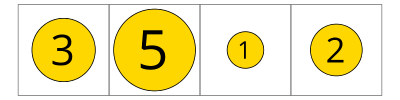
\includegraphics[width=3in]{img-1.png}
}

\end{figure}

Let's assume she chooses the 3 as it has a larger value. The coins now appear as

\begin{figure}[h]
\centerline {
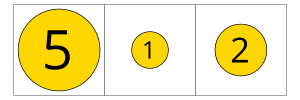
\includegraphics[width=3in]{img-2.png}
}

\end{figure}

The second player (Bob) may choose either the 5 or the 2, and will choose 5 as it is larger. We now have two remaining coins:

\begin{figure}[h]
\centerline {
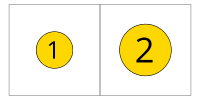
\includegraphics[width=2in]{img-3.png}
}

\end{figure}

Alice will choose the 2, and Bob will choose 1. The final score is Alice = 5 and Bob = 6.

So as you can see, having the first player initially choosing the highest-valued coin (known as a {\it greedy} algorithm) may not be an optimal strategy.  Instead, Alice should have initially chosen 2. Bob would have then chosen 3. Alice next chooses 5 and Bob chooses 1. Alice wins with a score of 7.

Design an algorithm that ensures the player that goes first can never lose. Rather, the first player will either win or tie. The goal of the game is not to get the optimal value of coins, but rather ensure the first player {\it never} loses. 

A few possible test cases (winning value is bold-faced.) 

10 5 {\bf 10} \\
3 5 1 2 {\bf 7} \\
8 9 8 5 5 0 {\bf 21} \\
83 50 14 11 39 79 1 25 {\bf 165}

 \end{document}
